\documentclass{article}
\usepackage[utf8]{inputenc}

%% Language and font encodings
\usepackage[english]{babel}
% \usepackage[utf8x]{inputenc}
\usepackage[T1]{fontenc}

%% Sets page size and margins
\usepackage[a4paper,top=2cm,bottom=2cm,left=2cm,right=2cm,marginparwidth=2cm]{geometry}

% %% for tabbing figures
% \usepackage{cuted}%%\stripsep-3pt
\usepackage{caption}
\usepackage{grffile}	% handle multi suffix (.drawio.png)
\usepackage{graphicx}
\usepackage{subfigure}  % multi-pictures in the same line

%% Sets row spaces
\usepackage{setspace}
\renewcommand{\baselinestretch}{1.0}

%% packages for tables
\usepackage{booktabs}

%% packages for tables
\usepackage{booktabs}

%% packages for code
\usepackage{xcolor}
\usepackage{listings}
\newcommand*{\listingautorefname}{Code}
\lstset{
	showstringspaces=false, %不显示中间的空格
}
\lstdefinestyle{lfonts}{
	basicstyle = \normalsize\ttfamily,
	stringstyle = \color{purple},
	keywordstyle = \color{blue!60!black}\bfseries,
	commentstyle = \color{olive}\scshape,
}
\lstdefinestyle{lnumbers}{
	numbers = left,
	numberstyle = \tiny,
	numbersep = 1em,
	firstnumber = 1,
	stepnumber = 1,
}
\lstdefinestyle{llayout}{
	breaklines = true,
	tabsize = 2,
	columns = flexible,
}
\lstdefinestyle{lgeometry}{
	xleftmargin = 20pt,
	xrightmargin = 0pt,
	frame = tb,
	framesep = \fboxsep,
	framexleftmargin = 20pt,
}
\lstdefinestyle{lgeneral}{
	style = lfonts,
	style = lnumbers,
	style = llayout,
	style = lgeometry,
}
\lstdefinestyle{python}{
	language = {Python},
	style = lgeneral,
}
\lstdefinestyle{shell}{
	language = {Shell},
	style = lgeneral,
}

%% packages for pseudocode
\usepackage{algorithm}
\usepackage{algorithmicx}  
\usepackage{algpseudocode}
\usepackage{amsmath}

%% packages for appendix
\usepackage[toc,page]{appendix}
\newcommand*{\Appendixautorefname}{Appendix}

%% Useful packages
\usepackage{amsmath}
\usepackage{graphicx}
\usepackage[colorinlistoftodos]{todonotes}
\usepackage[colorlinks=true, allcolors=blue]{hyperref}
\usepackage[numbers,sort&compress]{natbib} 
\usepackage{float}	% used for fix the location of tables and graphics
\usepackage{subfigure}  % multi-pictures in the same line
\newcommand{\upcite}[1]{\textsuperscript{\cite{#1}}}
\newcommand{\topcaption}{%
	\setlength{\abovecaptionskip}{0pt}%
	\setlength{\belowcaptionskip}{10pt}%
	\caption}

\title{\textbf{ECE329 Project \#1 Report}}
\author{Ruiqi Li, 3180111638}
\date{\today}

\begin{document}

%% for pseudo code
\renewcommand{\algorithmicrequire}{\textbf{Input:}}  % Use Input in the format of Algorithm
\renewcommand{\algorithmicensure}{\textbf{Output:}} % Use Output in the format of Algorithm
\newcommand{\algorithmautorefname}{Algorithm} % for hyperref

\maketitle

\section{Problem 1}

    \subsection{}

        The plot is shown as \autoref{fig:p1-1}.

        \begin{figure}[H]
            \centering
            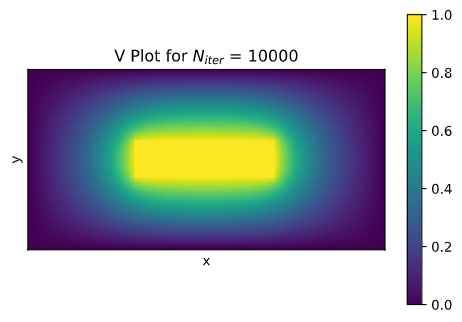
\includegraphics[width=0.6\textwidth]{img/p1_1.png}
            \caption{V over xy plane}
            \label{fig:p1-1}
        \end{figure}

    \subsection{}

        The plot is shown as \autoref{fig:p1-2}.

        \begin{figure}[H]
            \centering
            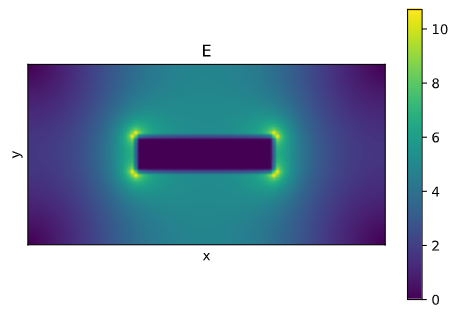
\includegraphics[width=0.6\textwidth]{img/p1_2.png}
            \caption{E over xy plane}
            \label{fig:p1-2}
        \end{figure}

        According to the code:

        \lstinputlisting[
            style = Python,
            firstline = 90,
            lastline = 96,
            caption = {Maxima of E},
            label = {code:p1-2}
        ]{../script/problem1.py}

        and its output:

        \begin{lstlisting}[style=Python]  
maxE = np.max(E)...
Points where E is at its maxima:
[[0.3  0.31]
 [0.69 0.31]
 [0.29 0.3 ]
 [0.7  0.3 ]
 [0.29 0.2 ]
 [0.7  0.2 ]
 [0.3  0.19]
 [0.69 0.19]]
        \end{lstlisting}

        We can find that the maxima of E field are focused on four corners of the rectangle.

    \subsection{}

        The plot is shown as \autoref{fig:p1-3}.

        \begin{figure}[H]
            \centering
            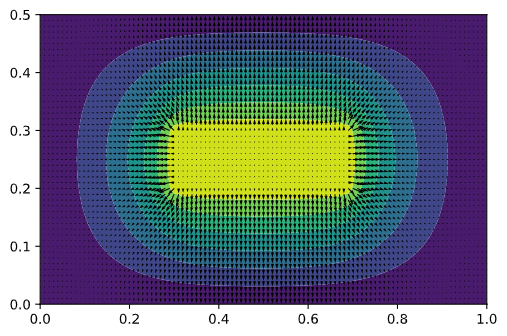
\includegraphics[width=0.6\textwidth]{img/p1_3.png}
            \caption{Contour of V and Vector Field of E}
            \label{fig:p1-3}
        \end{figure}

        The contour lines and the vectors in the vector field are perpendicular with each other.

    \subsection{}

        The plot of relative error of V is shown as \autoref{fig:p1-4}. The error is in log-scale.

        \begin{figure}[H]
            \centering
            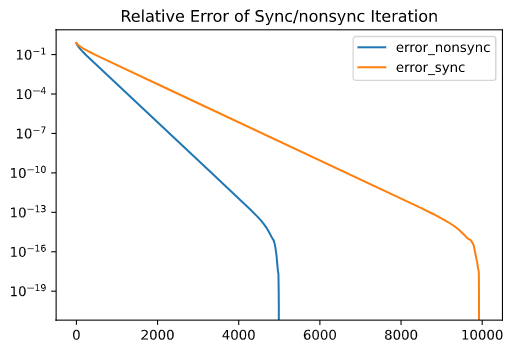
\includegraphics[width=0.6\textwidth]{img/p1_4.png}
            \caption{Relative Error of V of Sync/nonsync Iterations}
            \label{fig:p1-4}
        \end{figure}

\section{Problem 2}

    The plot is shown as \autoref{fig:p2-1}.

    \begin{figure}[H]
        \centering
        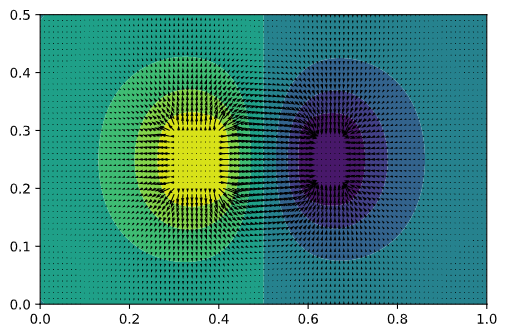
\includegraphics[width=0.6\textwidth]{img/p2_1.png}
        \caption{Contour of V and Vector Field of E for Problem 2}
        \label{fig:p2-1}
    \end{figure}

\end{document}
